\documentclass[aspectratio=43]{beamer}

% Theme and Color
\usetheme{CambridgeUS}
\usecolortheme{beaver}

% Additional Packages
\usepackage{amsmath, amssymb, amsfonts, graphicx, xcolor, hyperref}

% Title and Author
\title[\textbf{NCERT 9.1.4}]{Solving a Nonlinear Second-Order ODE}
\subtitle{\((\frac{d^2y}{dx^2})^2 + \cos\left(\frac{dy}{dx}\right) = 0\)}
\author[Krishna Patil]{EE24BTECH11036 \\ Krishna Patil}
\institute[University]{Department of Electrical Engineering}
\date{\today}

% Begin Document
\begin{document}

% Title Slide
\begin{frame}[plain]
    \titlepage
\end{frame}

% Outline Slide
\begin{frame}{Outline}
    \tableofcontents
\end{frame}

% Introduction Slide
\section{Introduction}
\begin{frame}{Introduction}
    \textbf{Problem Statement:} Solve the second-order nonlinear ODE:
    \[
    \left(\frac{d^2y}{dx^2}\right)^2 + \cos\left(\frac{dy}{dx}\right) = 0.
    \]
    \pause
    \textbf{Objective:}
    \begin{itemize}
        \item Convert the equation into a system of first-order ODEs.
        \item Apply the Runge-Kutta 4th-order method (RK4) for a numerical solution.
        \item Validate and visualize the results.
    \end{itemize}
\end{frame}

% System of First-Order ODEs Slide
\section{System of First-Order ODEs}
\begin{frame}{Converting to First-Order ODEs}
    Let:
    \[
    v = \frac{dy}{dx}, \quad u = \frac{d^2y}{dx^2}.
    \]
    The equation becomes:
    \[
    u^2 + \cos(v) = 0 \quad \implies \quad u = \pm \sqrt{-\cos(v)}.
    \]
    \pause
    The system of equations is:
    \begin{align*}
        \frac{dy}{dx} &= v, \\
        \frac{dv}{dx} &= u = \pm \sqrt{-\cos(v)}.
    \end{align*}
    \textbf{Note:} This is valid only when \( \cos(v) < 0 \).
\end{frame}

% RK4 Method Slide
\section{Runge-Kutta Method (RK4)}
\begin{frame}{Runge-Kutta 4th-Order Method (RK4)}
    \textbf{RK4 Method Overview:}
    \[
    y_{n+1} = y_n + \frac{1}{6}\left(k_1 + 2k_2 + 2k_3 + k_4\right),
    \]
    where
    \begin{align*}
        k_1 &= h \cdot f(x_n, y_n), \\
        k_2 &= h \cdot f\left(x_n + \frac{h}{2}, y_n + \frac{k_1}{2}\right), \\
        k_3 &= h \cdot f\left(x_n + \frac{h}{2}, y_n + \frac{k_2}{2}\right), \\
        k_4 &= h \cdot f(x_n + h, y_n + k_3).
    \end{align*}
    \pause
    Apply RK4 iteratively to approximate the solutions of the system:
    \begin{align*}
        \frac{dy}{dx} &= v, \quad \frac{dv}{dx} = \pm \sqrt{-\cos(v)}.
    \end{align*}
\end{frame}

% Numerical Solution Slide
\section{Numerical Solution}
\begin{frame}{Numerical Solution}
    Steps for numerical implementation:
    \begin{enumerate}
        \item Initialize \( y(0) = y_0 \) and \( v(0) = v_0 \) such that \( \cos(v_0) < 0 \).
        \item Choose a step size \( h \) (e.g., \( h = 0.01 \)).
        \item Iterate using RK4 to compute \( y_{n+1} \) and \( v_{n+1} \).
        \item Continue until the desired range of \( x \) is covered.
    \end{enumerate}
    \pause
    Example initial values:
    \[
    y(0) = 0, \quad v(0) = -1.
    \]
    Use these to compute the first few steps.
\end{frame}

% Visualization Slide
\section{Visualization}
\begin{frame}{Visualization of the Solution}
    \begin{figure}[h]
        \centering
        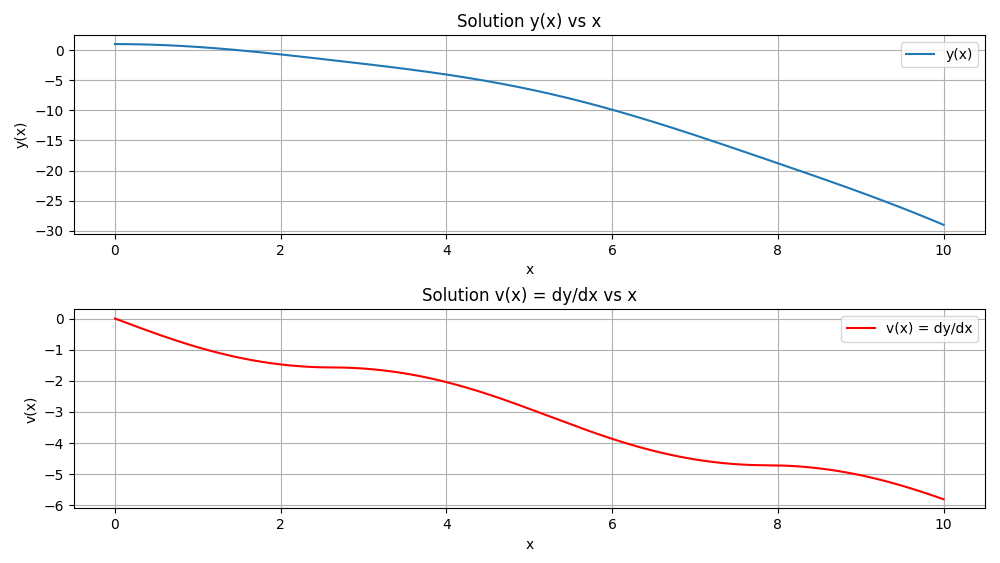
\includegraphics[width=0.8\linewidth]{fig/Figure_1.png}
        \caption{Numerical solution of the ODE.}
    \end{figure}
    \pause
    \textbf{Observation:} The solution satisfies the given ODE and respects the condition \( \cos(v) < 0 \).
\end{frame}

% Conclusion Slide
\section{Conclusion}
\begin{frame}{Conclusion}
    \textbf{Key Takeaways:}
    \begin{itemize}
        \item The given nonlinear second-order ODE can be converted into a system of first-order ODEs.
        \item The Runge-Kutta 4th-order method (RK4) is effective for solving such systems numerically.
        \item Visualizing the solution helps verify its accuracy and behavior.
    \end{itemize}
    \pause
    \textbf{Future Work:}
    \begin{itemize}
        \item Analyze the solution's behavior for different initial conditions.
        \item Extend the approach to similar nonlinear ODEs.
    \end{itemize}
\end{frame}

% Thank You Slide
\begin{frame}[plain]
    \centering
    \Huge \textbf{Thank You!}
\end{frame}

\end{document}

